\documentclass[11pt,a4paper]{article}
\usepackage[utf8]{inputenc}
\usepackage[T1]{fontenc}
\usepackage{textcomp}
\renewcommand{\tablename}{Tabla}\renewcommand{\figurename}{Figura}\renewcommand{\contentsname}{Índice}
\usepackage[margin=2.2cm]{geometry}
\usepackage{booktabs}
\usepackage{array}
\usepackage{amsmath,amssymb}
\usepackage{karnaugh-map}
\usepackage{circuitikz}
\usetikzlibrary{positioning,arrows.meta,calc}
\usepackage{caption}
\usepackage{subcaption}
\usepackage{float}
\usepackage{xcolor}
\usepackage{listings}
\usepackage{hyperref}
\usepackage{enumitem}

\hypersetup{colorlinks=true,linkcolor=blue!60!black,urlcolor=blue!60!black}
\captionsetup{font=small,labelfont=bf}
\setlength{\parskip}{3pt}
\setlength{\parindent}{0pt}
\lstset{basicstyle=\ttfamily\small,columns=fullflexible,keepspaces=true,frame=single,framerule=0.3pt,backgroundcolor=\color{gray!5},breaklines=true}

\newcommand{\bit}[1]{\texttt{#1}}
\newcommand{\sig}[1]{\texttt{#1}}
\newcommand{\nott}[1]{\overline{#1}}

\title{\textbf{Proyecto 1: Diseño Lógico y FPGA}\\[4pt]\Large Calculadora de 4 bits en complemento a dos}
\author{Arquitectura de Computadores \\ Universidad de los Andes \\ Semestre 2026-2 \\[6pt] \textit{Integrantes:} Nicolas Araneda \quad Vicente Calderon \quad Santiago Muñoz}
\date{8 de Septiembre de 2026}

\begin{document}
\maketitle

Este informe cubre los ítems 1 a 3 de la entrega: diseño general, tablas de verdad/Karnaugh/expresiones booleanas, e implementación mediante compuertas. El testbench, la simulación en GTKWave y el funcionamiento en la FPGA se muestran en la evaluación presencial. Todo el diseño está en \sig{src/} del repositorio; este documento sigue el mismo orden y los mismos nombres de módulo que el código.

\tableofcontents
\newpage

%=====================================================================
\section{Diseño general y arquitectura de la calculadora}
%=====================================================================

\subsection{Especificación}

La calculadora opera con números de 4 bits en complemento a dos (rango $-8$ a $+7$). Se mantuvo la codificación de operaciones del enunciado:

\begin{table}[H]
\centering
\begin{tabular}{@{}llll@{}}
\toprule
\textbf{Código} & \textbf{Operación} & \textbf{Resultado} & \textbf{Observación} \\
\midrule
\bit{000} & Reinicio      & $R = 0000$              & Ignora $A$ y $B$ \\
\bit{001} & Suma          & $R = A + B$             & Módulo 16 \\
\bit{010} & Resta         & $R = A - B$             & Complemento a dos, módulo 16 \\
\bit{011} & Resta inversa & $R = B - A$             & Complemento a dos, módulo 16 \\
\bit{100} & Shift left    & $R = A \ll B[1{:}0]$    & Lógico, rellena con ceros \\
\bit{101} & Shift right   & $R = A \gg B[1{:}0]$    & Lógico, rellena con ceros \\
\bit{110}, \bit{111} & inválido & $R = 0000$         & No alcanzables desde los botones \\
\bottomrule
\end{tabular}
\caption{Codificación de operaciones.}
\end{table}

Ningún archivo de \sig{src/} usa \bit{+ - < > <= >= << >> ?: if case}: toda la lógica combinacional está en primitivas de compuerta (\bit{and, or, not, xor, nand, nor, xnor, buf}). Lo único secuencial son los registros \bit{always @(posedge clk) q <= d;}, con \bit{d} calculado también con compuertas.

\subsection{Decisiones de diseño}

\begin{enumerate}[leftmargin=*,itemsep=2pt]
  \item \textbf{Aritmética módulo 16, sin detectar overflow.} El enunciado pide conservar los 4 bits menos significativos, así que el acarreo de salida del sumador se descarta directamente.
  \item \textbf{Resta con el mismo sumador.} $A-B = A+\nott{B}+1$. Una sola señal \sig{sub} invierte $B$ bit a bit (XOR) y entra como acarreo inicial del sumador. Suma, resta y resta inversa comparten \sig{adder4}.
  \item \textbf{Resta inversa por intercambio de operandos.} En vez de un segundo restador, ocho \sig{mux2} intercambian $A$ y $B$ cuando \sig{swap}=1 antes de restar.
  \item \textbf{Desplazamientos lógicos}, controlados solo por $B[1{:}0]$ como pide el enunciado; $B[3{:}2]$ se ignora.
  \item \textbf{Decodificador one-hot + enmascarado.} \sig{op\_decoder} entrega seis líneas one-hot; la ALU las usa como máscara AND/OR a la salida. Con un código inválido (\bit{110}, \bit{111}) las seis quedan en 0 y la salida es \bit{0000}: comportamiento seguro sin necesitar lógica extra.
  \item \textbf{Signo y magnitud en el display.} Izquierdo: guion si el valor es negativo. Derecho: magnitud en hexadecimal. Como $|V|\le 8$, los códigos 9--15 quedan disponibles como don't-care en el decodificador de 7 segmentos.
  \item \textbf{FSM de 2 bits.} Codificando los cuatro estados como contador binario, el próximo estado es $s_1\oplus s_0$ y $\nott{s_0}$: dos compuertas.
  \item \textbf{Debounce por muestreo.} 3 muestras iguales seguidas (a 1,31\,ms cada una) para aceptar un cambio, más detección de flanco para convertir el nivel en un pulso de un ciclo.
  \item \textbf{Reset de encendido.} Los cuatro botones ya están asignados por el enunciado; \sig{por} mantiene el reset activo 4 ciclos al partir para que la simulación no arranque en \bit{X}.
\end{enumerate}

\subsection{Arquitectura}

\begin{figure}[H]
\centering
\resizebox{\textwidth}{!}{%
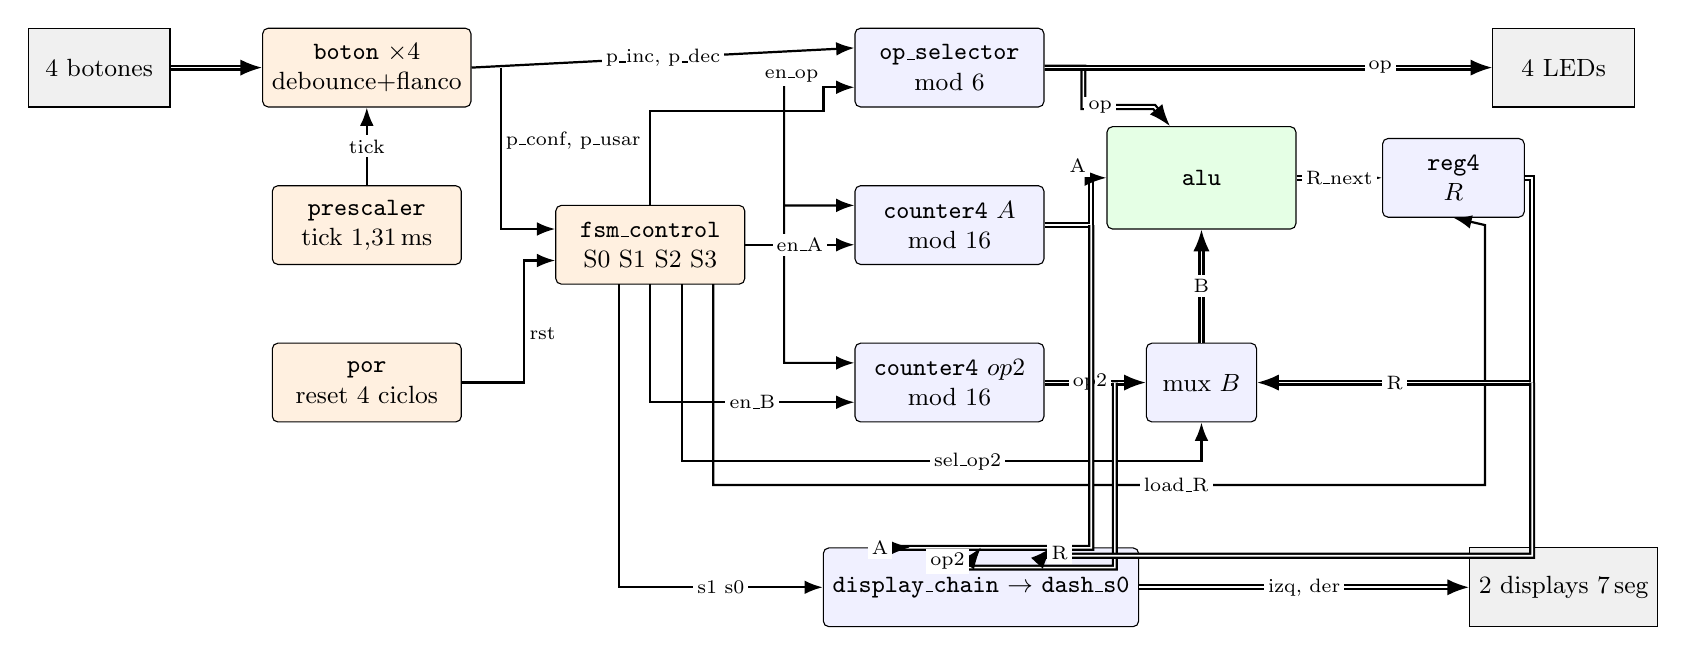
\begin{tikzpicture}[
  font=\small,
  blk/.style={draw,rounded corners=2pt,minimum height=10mm,minimum width=24mm,align=center,fill=blue!6},
  ctl/.style={draw,rounded corners=2pt,minimum height=10mm,minimum width=24mm,align=center,fill=orange!12},
  io/.style={draw,minimum height=10mm,minimum width=18mm,align=center,fill=gray!12},
  ar/.style={-Latex,thick},
  bus/.style={-Latex,thick,double},
  lbl/.style={font=\scriptsize,fill=white,inner sep=1.5pt}
]
\node[io]  (sw)  at (0,0)      {4 botones};
\node[ctl] (deb) at (3.4,0)    {\sig{boton} $\times4$\\debounce+flanco};
\node[ctl] (pre) at (3.4,-2)   {\sig{prescaler}\\tick 1,31\,ms};
\node[ctl] (por) at (3.4,-4)   {\sig{por}\\reset 4 ciclos};
\node[ctl] (fsm) at (7.0,-2.25){\sig{fsm\_control}\\S0 S1 S2 S3};
\node[blk] (ops) at (10.8,0)   {\sig{op\_selector}\\mod 6};
\node[blk] (ca)  at (10.8,-2)  {\sig{counter4} $A$\\mod 16};
\node[blk] (cb)  at (10.8,-4)  {\sig{counter4} $op2$\\mod 16};
\node[blk,minimum width=14mm] (mxb) at (14.0,-4) {mux $B$};
\node[blk,fill=green!10,minimum height=13mm] (alu) at (14.0,-1.4) {\sig{alu}};
\node[blk,minimum width=18mm] (reg) at (17.2,-1.4) {\sig{reg4}\\$R$};
\node[blk,minimum width=36mm] (disp) at (11.2,-6.6) {\sig{display\_chain} $\to$ \sig{dash\_s0}};
\node[io] (seg) at (18.6,-6.6) {2 displays 7\,seg};
\node[io] (led) at (18.6,0)    {4 LEDs};
\draw[bus] (sw) -- (deb);
\draw[ar]  (pre.north) -- node[lbl]{tick} (deb.south);
\draw[ar]  (deb.east) -- node[lbl,pos=0.5]{p\_inc, p\_dec} ($(ops.west)+(0,0.25)$);
\draw[ar]  (8.7,0) -- (8.7,-1.75) -- ($(ca.west)+(0,0.25)$);
\draw[ar]  (8.7,-1.75) -- (8.7,-3.75) -- ($(cb.west)+(0,0.25)$);
\draw[ar]  (5.1,0) -- node[lbl,pos=0.45,right]{p\_conf, p\_usar} (5.1,-2.05) -- ($(fsm.west)+(0,0.2)$);
\draw[ar]  (por.east) -- (5.4,-4) -- node[lbl,pos=0.4,right]{rst} (5.4,-2.45) -- ($(fsm.west)+(0,-0.2)$);
\draw[ar]  (fsm.north) -- (7.0,-0.55) -- (9.2,-0.55) -- (9.2,-0.25) -- node[lbl,pos=0.0,above left]{en\_op} ($(ops.west)+(0,-0.25)$);
\draw[ar]  (fsm.east) -- node[lbl]{en\_A} ($(ca.west)+(0,-0.25)$);
\draw[ar]  (7.0,-2.75) -- (7.0,-4.25) -- node[lbl,pos=0.5]{en\_B} ($(cb.west)+(0,-0.25)$);
\draw[ar]  (6.6,-2.75) -- (6.6,-6.6) -- node[lbl,pos=0.5]{s1 s0} (disp.west);
\draw[ar]  (7.4,-2.75) -- (7.4,-5.0) -- node[lbl,pos=0.55]{sel\_op2} (14.0,-5.0) -- (mxb.south);
\draw[ar]  (7.8,-2.75) -- (7.8,-5.3) -- node[lbl,pos=0.6]{load\_R} (17.6,-5.3) -- (17.6,-2.0) -- (reg.south);
\draw[bus] (ops.east) -- (12.5,0) -- (12.5,-0.5) -- node[lbl,pos=0.0,right]{op} (13.4,-0.5) -- ($(alu.north)+(-0.4,0)$);
\draw[bus] (ops.east) -- node[lbl,pos=0.75]{op} (led.west);
\draw[bus] (ca.east) -- (12.6,-2) -- (12.6,-1.4) -- node[lbl,pos=0.0,above left]{A} (alu.west);
\draw[bus] (cb.east) -- node[lbl,pos=0.45]{op2} (mxb.west);
\draw[bus] (mxb.north) -- node[lbl]{B} (alu.south);
\draw[bus] (alu.east) -- node[lbl]{R\_next} (reg.west);
\draw[bus] (reg.east) -- (18.2,-1.4) -- (18.2,-4) -- node[lbl,pos=0.5]{R} (mxb.east);
\draw[bus] (12.6,-2) -- (12.6,-6.1) -- (10.0,-6.1) -- node[lbl,pos=0.3,left]{A} ($(disp.north)+(-0.9,0)$);
\draw[bus] (12.9,-4) -- (12.9,-6.35) -- (11.0,-6.35) -- node[lbl,pos=0.3,left]{op2} (disp.north);
\draw[bus] (18.2,-4) -- (18.2,-6.2) -- (12.0,-6.2) -- node[lbl,pos=0.3,right]{R} ($(disp.north)+(0.9,0)$);
\draw[bus] (disp) -- node[lbl]{izq, der} (seg);
\end{tikzpicture}}
\caption{Diagrama de bloques (módulo \sig{top}). Naranjo: control e interfaz de botones. Azul: camino de datos. Verde: ALU combinacional.}
\label{fig:bloques}
\end{figure}

\sig{op\_selector} no tiene entrada de habilitación propia, así que \sig{top} filtra sus pulsos de entrada con \sig{en\_op} (dos \bit{and}, \sig{go1}/\sig{go2}) antes de conectarlos: sin ese filtro, subir en cualquier otro estado también cambiaría la operación.

\subsection{Los dos módulos de nivel superior}

Hay dos módulos que comparten el mismo núcleo (\sig{alu} + \sig{reg4}/\sig{reg4\_ini}):

\begin{table}[H]
\centering
\small
\begin{tabular}{@{}lp{6.2cm}p{6.2cm}@{}}
\toprule
 & \textbf{\sig{top}} & \textbf{\sig{calculadora\_4bits}} \\
\midrule
Entradas & 4 botones físicos & \sig{codigo}, \sig{op1}, \sig{op2\_ext}, \sig{sel\_op2}, \sig{ejecutar} directos \\
Control & FSM de 4 estados + debounce & una sola señal \sig{ejecutar} \\
Salida & LEDs + 2 displays de 7 segmentos & \sig{resultado} de 4 bits, sin decodificar \\
\bottomrule
\end{tabular}
\caption{\sig{top} es la calculadora en la placa. \sig{calculadora\_4bits} es el envoltorio con la interfaz que usará el testbench de la evaluación (mismo \sig{codigo} de 3 bits, mismo \sig{op1}/\sig{op2\_ext} de 4 bits y el mismo selector de segundo operando de 1 bit que pide el enunciado). No reimplementa nada: instancia la misma \sig{alu}.}
\end{table}

\sig{calculadora\_4bits} usa \sig{reg4\_ini} en vez de \sig{reg4}: es el mismo registro pero sin puerto de reset (la interfaz de la evaluación no lo tiene) y con valor inicial \bit{0000} en la declaración del flip-flop en su lugar.

\subsection{Interfaz de usuario y máquina de estados}

\begin{table}[H]
\centering
\begin{tabular}{@{}lll@{}}
\toprule
\textbf{Botón} & \textbf{Puerto} & \textbf{Función} \\
\midrule
Superior izquierdo & \sig{i\_Switch\_1} & Incrementar \\
Inferior izquierdo & \sig{i\_Switch\_2} & Disminuir \\
Superior derecho   & \sig{i\_Switch\_3} & Confirmar / avanzar de estado \\
Inferior derecho   & \sig{i\_Switch\_4} & Usar el resultado anterior como segundo operando \\
\bottomrule
\end{tabular}
\caption{Asignación de botones (Nandland Go Board).}
\end{table}

\begin{figure}[H]
\centering
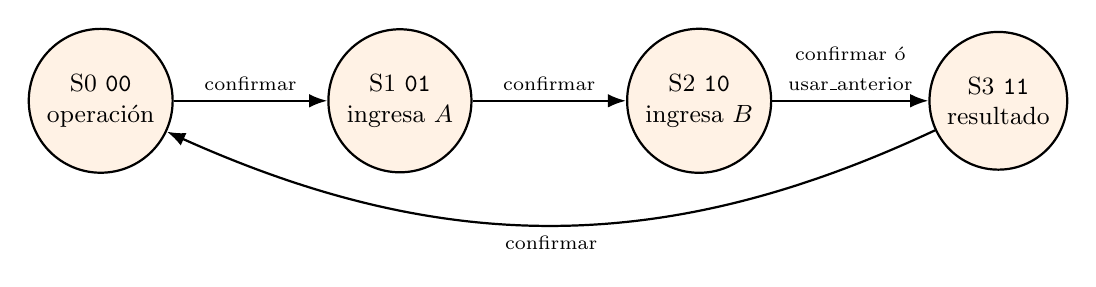
\begin{tikzpicture}[font=\small,node distance=38mm,
  st/.style={draw,circle,minimum size=15mm,align=center,fill=orange!10,thick},
  ar/.style={-Latex,thick}]
\node[st] (s0) {S0 \bit{00}\\operación};
\node[st,right of=s0] (s1) {S1 \bit{01}\\ingresa $A$};
\node[st,right of=s1] (s2) {S2 \bit{10}\\ingresa $B$};
\node[st,right of=s2] (s3) {S3 \bit{11}\\resultado};
\draw[ar] (s0) -- node[above]{\scriptsize confirmar} (s1);
\draw[ar] (s1) -- node[above]{\scriptsize confirmar} (s2);
\draw[ar] (s2) -- node[above,align=center]{\scriptsize confirmar ó\\\scriptsize usar\_anterior} (s3);
\draw[ar] (s3) to[bend left=25] node[below]{\scriptsize confirmar} (s0);
\end{tikzpicture}
\caption{Máquina de estados de control (\sig{fsm\_control}).}
\label{fig:fsm}
\end{figure}

\begin{table}[H]
\centering
\small
\begin{tabular}{@{}cccp{3.6cm}p{3.6cm}@{}}
\toprule
$s_1s_0$ & \textbf{Estado} & \textbf{Habilita} & \textbf{Botones izquierdos} & \textbf{Displays} \\
\midrule
00 & S0 & \sig{en\_op} & cambian el código de operación & guion en ambos \\
01 & S1 & \sig{en\_A}  & cambian $A$ & signo + magnitud de $A$ \\
10 & S2 & \sig{en\_B}  & cambian $op2$ & signo + magnitud de $op2$ \\
11 & S3 & \sig{en\_R}  & sin efecto & signo + magnitud de $R$ \\
\bottomrule
\end{tabular}
\caption{Comportamiento por estado. \sig{op}[2] es el LED 1 (bit más significativo).}
\end{table}

En S2, si se presiona el botón inferior derecho, \sig{sel\_op2} (combinacional: \sig{usar\_anterior} \verb|AND| \sig{en\_B}) hace que el mux de $B$ tome $R$ en vez de $op2$, y \sig{load\_R} carga el resultado en el mismo ciclo. La realimentación $R\to$ mux $\to$ ALU $\to$ \sig{reg4} $\to R$ no es un lazo combinacional porque el flip-flop de \sig{reg4} corta el camino. Los operandos $A$ y $op2$ no se reinician entre rondas; para poner el resultado en 0 se usa la operación \bit{000}.

\subsection{Interfaz física y polaridad}

\begin{itemize}[leftmargin=*,itemsep=1pt]
  \item \textbf{Reloj:} oscilador de 25\,MHz de la placa.
  \item \textbf{Botones y LEDs:} activos en alto. Entran por cuatro \bit{buf} en \sig{top.v}; si la polaridad resultara ser la contraria, se cambian esos cuatro \bit{buf} por \bit{not} y no hay que tocar nada más.
  \item \textbf{Displays de 7 segmentos (5261BG):} ánodo común, activos en \textbf{bajo}, verificado directamente en la placa. Toda la lógica interna sigue en lógica positiva; las 14 salidas de segmento pasan por un \bit{not} final. Es De Morgan aplicado en la salida y no obliga a rehacer ningún mapa de Karnaugh.
  \item \textbf{Formato de bus:} \sig{seg[6:0]} $=\{a,b,c,d,e,f,g\}$.
\end{itemize}

\subsection{Verificación}

\begin{table}[H]
\centering
\small
\begin{tabular}{@{}lll@{}}
\toprule
\textbf{Testbench} & \textbf{Casos} & \textbf{Resultado} \\
\midrule
\sig{adder4\_tb}            & 512 (barrido exhaustivo, $16\times16\times2$) & Sin errores \\
\sig{shifter\_tb}           & 64 por dirección (exhaustivo)                 & Sin errores \\
\sig{op\_selector\_tb}      & 19 (subida, bajada, retención, prioridad, reset) & Sin errores \\
\sig{alu\_tb}                & 2\,048 (exhaustivo, $8\times16\times16$)      & Sin errores \\
\sig{display\_tb}           & 107 (\sig{abs4}, \sig{seg7\_decoder}, mux de fuente) & Sin errores \\
\sig{debounce\_tb}          & 11 (prescaler, rebote, glitch, flanco)        & Sin errores \\
\sig{control\_tb}           & 79 (contadores, registro, FSM, one-hot)       & Sin errores \\
\sig{calculadora\_4bits\_tb} & 17 (interfaz de la evaluación)                & Sin errores \\
\sig{top\_tb}                & 33 (punta a punta, pulsaciones reales)        & Sin errores \\
\sig{demo\_tb}, \sig{alu\_wave\_tb} & editables, para la evaluación presencial & -- \\
\bottomrule
\end{tabular}
\caption{Cobertura de simulación (Icarus Verilog). \sig{alu\_tb} verifica además que el decodificador se mantenga one-hot y que \bit{110}/\bit{111} dejen las seis salidas en 0.}
\end{table}

Los once testbenches propios tampoco usan \bit{if} ni \bit{case}: para contar errores se usa que \bit{(obtenido !== esperado)} entrega 1 ó 0 y se acumula directo, y el veredicto final se imprime indexando un arreglo de strings con esa bandera. Los operadores aritméticos sólo aparecen ahí, para calcular el valor de referencia contra el que se compara el diseño de compuertas.

\textbf{Síntesis} (yosys 0.68 + nextpnr-ice40, iCE40 HX1K VQ100): 174 celdas lógicas de 1\,280 (13\,\%), 56 flip-flops, 23 pines de 72 (31\,\%). La netlist son 166 \sig{SB\_LUT4} + 56 \sig{SB\_DFF}. Frecuencia máxima 122,31\,MHz tras el ruteo, contra los 25\,MHz del oscilador de la placa. Sin latches inferidos ni lazos combinacionales.

\newpage
%=====================================================================
\section{Tablas de verdad, mapas de Karnaugh y expresiones booleanas}
%=====================================================================

Convención: $\nott{x}$ es la negación, la yuxtaposición es AND, $+$ es OR, $\oplus$ es XOR. Los bloques que se arman por composición jerárquica de un mux2 o un sumador de 1 bit (barrel shifters, mux de $B$, mux de fuente del display) no llevan un mapa de Karnaugh de múltiples entradas propio: se documenta la tabla de la celda base y cómo se replica, en vez de un mapa de 6 entradas que no simplificaría nada y sería ilegible.

\subsection{Multiplexor 2:1 (\sig{mux2})}

\begin{minipage}[t]{0.4\textwidth}
\vspace{0pt}\centering
\begin{tabular}{@{}ccc|c@{}}
\toprule
$sel$ & $d_1$ & $d_0$ & $y$ \\
\midrule
0&0&0&0\\ 0&0&1&1\\ 0&1&0&0\\ 0&1&1&1\\
1&0&0&0\\ 1&0&1&0\\ 1&1&0&1\\ 1&1&1&1\\
\bottomrule
\end{tabular}
\end{minipage}
\begin{minipage}[t]{0.55\textwidth}
\vspace{0pt}\centering
\begin{karnaugh-map}[4][2][1][$d_1d_0$][$sel$]
\minterms{1,3,6,7}
\implicant{1}{3}
\implicant{7}{6}
\end{karnaugh-map}
\end{minipage}

\[ y = \nott{sel}\,d_0 + sel\,d_1 \]

SOP mínima, no simplificable más (dos implicantes primos esenciales, sin consenso útil). 4 compuertas: 1 NOT + 2 AND + 1 OR. Es el bloque más instanciado del diseño: aparece en swap, shifters, mux de $B$, mux de fuente del display, y en todos los registros con retención (FSM, contadores, \sig{reg4}, debounce).

\subsection{Sumador completo de 1 bit (\sig{full\_adder})}

\begin{minipage}[t]{0.36\textwidth}
\vspace{0pt}\centering
\begin{tabular}{@{}ccc|cc@{}}
\toprule
$a$ & $b$ & $c_{in}$ & $s$ & $c_{out}$ \\
\midrule
0&0&0&0&0\\ 0&0&1&1&0\\ 0&1&0&1&0\\ 0&1&1&0&1\\
1&0&0&1&0\\ 1&0&1&0&1\\ 1&1&0&0&1\\ 1&1&1&1&1\\
\bottomrule
\end{tabular}
\end{minipage}
\begin{minipage}[t]{0.3\textwidth}
\vspace{0pt}\centering
$s$\\
\begin{karnaugh-map}[4][2][1][$b\,c_{in}$][$a$]
\minterms{1,2,4,7}
\end{karnaugh-map}
\end{minipage}
\begin{minipage}[t]{0.3\textwidth}
\vspace{0pt}\centering
$c_{out}$\\
\begin{karnaugh-map}[4][2][1][$b\,c_{in}$][$a$]
\minterms{3,5,6,7}
\implicant{3}{7}\implicant{5}{7}\implicant{7}{6}
\end{karnaugh-map}
\end{minipage}

\[ s = a \oplus b \oplus c_{in} \qquad c_{out} = ab + a\,c_{in} + b\,c_{in} = ab + (a\oplus b)\,c_{in} \]

El mapa de $s$ es un tablero de ajedrez (función XOR, sin implicantes de más de una celda). La forma implementada de $c_{out}$ reutiliza $a\oplus b$, ya calculado para $s$: 2 XOR + 2 AND + 1 OR = 5 compuertas en vez de las 6 que saldrían de tomar los tres implicantes primos por separado.

\subsection{Sumador de 4 bits (\sig{adder4})}

Cuatro \sig{full\_adder} en cadena (ripple-carry): $s_i = a_i\oplus b_i\oplus c_i$, $c_{i+1} = a_ib_i + (a_i\oplus b_i)c_i$, $c_0 = c_{in}$. El acarreo $c_4$ se descarta, lo que da directamente la aritmética módulo 16 pedida. 20 compuertas (4$\times$5). Verificado con las 512 combinaciones de $a$, $b$, $c_{in}$.

\subsection{Acondicionador de resta}

$A-B = A+\nott{B}+1$ (módulo 16). Con una señal \sig{sub}:

\begin{minipage}[t]{0.4\textwidth}
\vspace{0pt}\centering
\begin{tabular}{@{}cc|c@{}}
\toprule
\sig{sub} & $y_i$ & $y^c_i$ \\
\midrule
0&0&0\\ 0&1&1\\ 1&0&1\\ 1&1&0\\
\bottomrule
\end{tabular}
\end{minipage}
\begin{minipage}[t]{0.5\textwidth}
\vspace{0pt}
\[ y^c_i = y_i \oplus \mathit{sub}, \qquad c_{in} = \mathit{sub} \]
\end{minipage}

Con \sig{sub}=0 el operando pasa intacto y $c_{in}=0$ (suma). Con \sig{sub}=1 se invierte cada bit y el mismo \sig{sub} entra como acarreo inicial, aportando el $+1$ del complemento a dos: 4 XOR, sin restador aparte.

\subsection{Decodificador de operación (\sig{op\_decoder})}
\label{sec:decoder}

\begin{table}[H]
\centering
\begin{tabular}{@{}ccc|cccccc@{}}
\toprule
$op_2$&$op_1$&$op_0$ & \sig{sel\_rst}&\sig{sel\_add}&\sig{sel\_sub}&\sig{sel\_rsub}&\sig{sel\_shl}&\sig{sel\_shr} \\
\midrule
0&0&0& 1&0&0&0&0&0 \\
0&0&1& 0&1&0&0&0&0 \\
0&1&0& 0&0&1&0&0&0 \\
0&1&1& 0&0&0&1&0&0 \\
1&0&0& 0&0&0&0&1&0 \\
1&0&1& 0&0&0&0&0&1 \\
1&1&0& 0&0&0&0&0&0 \\
1&1&1& 0&0&0&0&0&0 \\
\bottomrule
\end{tabular}
\caption{\bit{110} y \bit{111} son códigos inválidos: las seis salidas quedan en 0.}
\end{table}

Cada salida es exactamente un mintérmino de tres literales:
\[
\begin{aligned}
\mathit{sel\_rst}  &= \nott{op_2}\nott{op_1}\nott{op_0} &
\mathit{sel\_add}  &= \nott{op_2}\nott{op_1}op_0 &
\mathit{sel\_sub}  &= \nott{op_2}op_1\nott{op_0} \\
\mathit{sel\_rsub} &= \nott{op_2}op_1op_0 &
\mathit{sel\_shl}  &= op_2\nott{op_1}\nott{op_0} &
\mathit{sel\_shr}  &= op_2\nott{op_1}op_0
\end{aligned}
\]

\bit{110} y \bit{111} podrían tratarse como don't-care: por ejemplo $\mathit{sel\_shl}$ se reduciría a $op_2\nott{op_0}$ (Figura~\ref{fig:kmap-dec}). Se decidió \textbf{no aprovecharlos}: con las expresiones completas, un código inválido deja las seis líneas en 0 y la ALU entrega \bit{0000}, además de garantizar que el decodificador sea one-hot (lo que necesita el enmascarado de salida de la ALU, sección~\ref{sec:alu-impl}). El costo es una entrada más en dos de las seis compuertas AND.

\begin{figure}[H]
\centering
\begin{subfigure}[t]{0.32\textwidth}\centering
\begin{karnaugh-map}[4][2][1][$op_1op_0$][$op_2$]
\minterms{4}\indeterminants{6,7}\implicant{4}{4}
\end{karnaugh-map}
\caption{Sin aprovechar don't-care: $op_2\nott{op_1}\nott{op_0}$}
\end{subfigure}\hfill
\begin{subfigure}[t]{0.32\textwidth}\centering
\begin{karnaugh-map}[4][2][1][$op_1op_0$][$op_2$]
\minterms{4}\indeterminants{6,7}\implicantedge{4}{4}{6}{6}
\end{karnaugh-map}
\caption{Aprovechándolos: $op_2\nott{op_0}$ (descartada)}
\end{subfigure}\hfill
\begin{subfigure}[t]{0.32\textwidth}\centering
\begin{karnaugh-map}[4][2][1][$op_1op_0$][$op_2$]
\minterms{2,3}\indeterminants{6,7}\implicant{3}{2}
\end{karnaugh-map}
\caption{$\mathit{sub}=\nott{op_2}\,op_1$}
\end{subfigure}
\caption{\sig{sel\_shl} con y sin don't-care, y la señal derivada \sig{sub}.}
\label{fig:kmap-dec}
\end{figure}

Las señales de control de la ALU se derivan de las líneas ya decodificadas:
\[ \mathit{sub} = \mathit{sel\_sub} + \mathit{sel\_rsub} = \nott{op_2}\,op_1, \qquad \mathit{swap} = \mathit{sel\_rsub}. \]
En el código, \sig{sub} es un OR de dos líneas que ya existen (una compuerta), equivalente a la expresión mínima.

\subsection{Intercambio de operandos y barrel shifters}

Para $B-A$ se reutiliza la resta $x-y$ intercambiando las entradas con ocho \sig{mux2}: $x_i = \nott{\mathit{swap}}\,a_i + \mathit{swap}\,b_i$, $y_i = \nott{\mathit{swap}}\,b_i + \mathit{swap}\,a_i$. Los shifters operan sobre $A$ directo, no sobre $x$: el intercambio sólo afecta la vía aritmética.

Un desplazamiento de 0 a 3 posiciones se arma en dos etapas de \sig{mux2} (desplaza 1 si $sh_0$, desplaza 2 si $sh_1$), rellenando con 0 las posiciones que quedan vacías:

\begin{table}[H]
\centering
\begin{subtable}[t]{0.48\textwidth}\centering
\begin{tabular}{@{}c|cccc@{}}
\toprule
$sh_0$ & $t_3$ & $t_2$ & $t_1$ & $t_0$ \\
\midrule
0 & $a_3$ & $a_2$ & $a_1$ & $a_0$ \\ 1 & $a_2$ & $a_1$ & $a_0$ & 0 \\
\bottomrule
\end{tabular}\vspace{2pt}
\begin{tabular}{@{}c|cccc@{}}
\toprule
$sh_1$ & $y_3$ & $y_2$ & $y_1$ & $y_0$ \\
\midrule
0 & $t_3$ & $t_2$ & $t_1$ & $t_0$ \\ 1 & $t_1$ & $t_0$ & 0 & 0 \\
\bottomrule
\end{tabular}
\caption{Shift left}
\end{subtable}\hfill
\begin{subtable}[t]{0.48\textwidth}\centering
\begin{tabular}{@{}c|cccc@{}}
\toprule
$sh_0$ & $t_3$ & $t_2$ & $t_1$ & $t_0$ \\
\midrule
0 & $a_3$ & $a_2$ & $a_1$ & $a_0$ \\ 1 & 0 & $a_3$ & $a_2$ & $a_1$ \\
\bottomrule
\end{tabular}\vspace{2pt}
\begin{tabular}{@{}c|cccc@{}}
\toprule
$sh_1$ & $y_3$ & $y_2$ & $y_1$ & $y_0$ \\
\midrule
0 & $t_3$ & $t_2$ & $t_1$ & $t_0$ \\ 1 & 0 & 0 & $t_3$ & $t_2$ \\
\bottomrule
\end{tabular}
\caption{Shift right}
\end{subtable}
\caption{Tablas por etapa de los barrel shifters ($sh=B[1{:}0]$).}
\end{table}

Los muxes con una entrada 0 se reducen a un AND ($\nott{sh}\cdot a$) en síntesis. 8 \sig{mux2} por dirección = 32 compuertas cada uno.

\subsection{Selector de operación: contador módulo 6 (\sig{op\_selector})}

El estado $q_2q_1q_0$ recorre \bit{000}$\to\cdots\to$\bit{101}$\to$\bit{000} al subir y al revés al bajar; \bit{110} y \bit{111} son don't-care porque nunca se alcanzan.

\begin{table}[H]
\centering
\begin{tabular}{@{}ccc|ccc|ccc@{}}
\toprule
\multicolumn{3}{c|}{Estado} & \multicolumn{3}{c|}{Subir} & \multicolumn{3}{c}{Bajar} \\
$q_2$&$q_1$&$q_0$ & $n_2$&$n_1$&$n_0$ & $n_2$&$n_1$&$n_0$ \\
\midrule
0&0&0 & 0&0&1 & 1&0&1 \\ 0&0&1 & 0&1&0 & 0&0&0 \\
0&1&0 & 0&1&1 & 0&0&1 \\ 0&1&1 & 1&0&0 & 0&1&0 \\
1&0&0 & 1&0&1 & 0&1&1 \\ 1&0&1 & 0&0&0 & 1&0&0 \\
1&1&0 & --&--&-- & --&--&-- \\ 1&1&1 & --&--&-- & --&--&-- \\
\bottomrule
\end{tabular}
\caption{Próximo estado del selector de operación.}
\end{table}

\begin{figure}[H]
\centering
\begin{subfigure}[t]{0.32\textwidth}\centering
\begin{karnaugh-map}[4][2][1][$q_1q_0$][$q_2$]
\minterms{0,2,4}\indeterminants{6,7}\implicantedge{0}{4}{2}{6}
\end{karnaugh-map}
\caption{$n_0$ (ambos sentidos) $=\nott{q_0}$}
\end{subfigure}
\begin{subfigure}[t]{0.32\textwidth}\centering
\begin{karnaugh-map}[4][2][1][$q_1q_0$][$q_2$]
\minterms{1,2}\indeterminants{6,7}\implicant{1}{1}\implicant{2}{2}
\end{karnaugh-map}
\caption{$n_1$ subir $=\nott{q_2}(q_1\oplus q_0)$}
\end{subfigure}
\begin{subfigure}[t]{0.32\textwidth}\centering
\begin{karnaugh-map}[4][2][1][$q_1q_0$][$q_2$]
\minterms{3,4}\indeterminants{6,7}\implicant{3}{7}\implicantedge{4}{4}{6}{6}
\end{karnaugh-map}
\caption{$n_2$ subir $=q_1q_0+q_2\nott{q_0}$}
\end{subfigure}
\caption{Mapas de Karnaugh del contador módulo 6 (subida). Bajada es análoga.}
\end{figure}

Expresiones mínimas (aprovechando los don't-care):
\[
\begin{aligned}
\text{subir:}&& n_0&=\nott{q_0}, & n_1&=\nott{q_2}(q_1\oplus q_0), & n_2&=q_1q_0+q_2\nott{q_0},\\
\text{bajar:}&& n_0&=\nott{q_0}, & n_1&=q_1q_0+q_2\nott{q_0}, & n_2&=\nott{q_1}(q_2\odot q_0).
\end{aligned}
\]

\textbf{Nota de consistencia.} El código no usa exactamente estas formas mínimas para la bajada: implementa $n_1=\nott{q_2}q_1q_0+q_2\nott{q_1}\nott{q_0}$ y $n_2=\nott{q_2}\nott{q_1}\nott{q_0}+q_2\nott{q_1}q_0$, la forma de mintérminos completos (sin aprovechar los don't-care). Ambas formas son funcionalmente equivalentes en los seis estados alcanzables, verificado en \sig{op\_selector\_tb}; se prefirió la forma completa por la misma razón que en el decodificador de operación: si el registro cayera en \bit{110} o \bit{111} por algún transitorio, esta forma lo devuelve a un estado válido en un ciclo.

\subsection{Contador módulo 16 (\sig{counter4})}

Aquí el módulo 16 es el desborde natural de 4 bits: no hace falta lógica de vuelta, sólo descartar el acarreo/préstamo de salida.

\begin{center}
\begin{tabular}{@{}cc|cc@{}}
\toprule
$q_i$ & $c_i$ & $n_i$ & $c_{i+1}$ \\
\midrule
0&0&0&0\\ 0&1&1&0\\ 1&0&1&0\\ 1&1&0&1\\
\bottomrule
\end{tabular}
\qquad
\begin{tabular}{@{}cc|cc@{}}
\toprule
$q_i$ & $b_i$ & $n_i$ & $b_{i+1}$ \\
\midrule
0&0&0&0\\ 0&1&1&1\\ 1&0&1&0\\ 1&1&0&0\\
\bottomrule
\end{tabular}
\end{center}

\[
\text{subir: } n_i=q_i\oplus c_i,\ c_{i+1}=c_i q_i,\ c_0=1
\qquad
\text{bajar: } n_i=q_i\oplus b_i,\ b_{i+1}=b_i\nott{q_i},\ b_0=1
\]

Con $c_0=b_0=1$, el bit 0 queda igual en los dos sentidos ($n_0=\nott{q_0}$) y $c_1=q_0$, $b_1=\nott{q_0}$ salen sin compuertas adicionales: una sola señal se comparte. La misma cadena de acarreo (sólo la de subida, 15 bits) es el \sig{prescaler}: $\mathit{tick}=c_{15}=q_{14}q_{13}\cdots q_0$, o sea el contador en todos unos, sin necesitar comparador.

\subsection{Máquina de estados de control (\sig{fsm\_control})}

\begin{table}[H]
\centering
\begin{tabular}{@{}cc|cc|cccc@{}}
\toprule
$s_1$&$s_0$ & $n_1$&$n_0$ & \sig{en\_op}&\sig{en\_A}&\sig{en\_B}&\sig{en\_R}\\
\midrule
0&0 & 0&1 & 1&0&0&0\\
0&1 & 1&0 & 0&1&0&0\\
1&0 & 1&1 & 0&0&1&0\\
1&1 & 0&0 & 0&0&0&1\\
\bottomrule
\end{tabular}
\caption{Próximo estado (si \sig{avanzar}=1) y decodificación one-hot.}
\end{table}

Con esta codificación binaria, $s_0s_1s_2s_3\to$ recorrer los cuatro estados es contar en binario: $n_1=s_1\oplus s_0$, $n_0=\nott{s_0}$ (no requiere mapa de Karnaugh, sale directo de la tabla). Señales de control, todas combinacionales:
\[
\begin{aligned}
\mathit{en\_B} &= s_1\nott{s_0} \ (\text{detecta S2}) &
\mathit{sel\_op2} &= \mathit{usar\_anterior}\cdot\mathit{en\_B} \\
\mathit{load\_R} &= \mathit{en\_B}\cdot(\mathit{confirmar}+\mathit{usar\_anterior}) &
\mathit{avanzar} &= \mathit{confirmar}+\mathit{sel\_op2}
\end{aligned}
\]
La retención (sin pulso, el estado se mantiene) usa un \sig{mux2} por bit: $d_1=\mathit{avanzar}\,n_1+\nott{\mathit{avanzar}}\,s_1$, análogo para $d_0$.

\subsection{Signo y valor absoluto (\sig{abs4})}

$\mathit{signo}=V_3$; $|V|=(V\oplus V_3)+V_3$ (el bit 3 del XOR es $V_3\oplus V_3=0$ siempre, así que son 3 XOR, no 4, más una instancia de \sig{adder4} con $c_{in}=V_3$).

\begin{table}[H]
\centering\small
\begin{tabular}{@{}cccc|c|c@{}}
\toprule
$V_3V_2V_1V_0$ & valor & signo & $D_3D_2D_1D_0$ & $|V|$ \\
\midrule
0000 & 0 & 0 & 0000 & 0\\ 0001 & 1 & 0 & 0001 & 1\\ 0010 & 2 & 0 & 0010 & 2\\ 0011 & 3 & 0 & 0011 & 3\\
0100 & 4 & 0 & 0100 & 4\\ 0101 & 5 & 0 & 0101 & 5\\ 0110 & 6 & 0 & 0110 & 6\\ 0111 & 7 & 0 & 0111 & 7\\
1000 & $-8$ & 1 & 1000 & 8\\ 1001 & $-7$ & 1 & 0111 & 7\\ 1010 & $-6$ & 1 & 0110 & 6\\ 1011 & $-5$ & 1 & 0101 & 5\\
1100 & $-4$ & 1 & 0100 & 4\\ 1101 & $-3$ & 1 & 0011 & 3\\ 1110 & $-2$ & 1 & 0010 & 2\\ 1111 & $-1$ & 1 & 0001 & 1\\
\bottomrule
\end{tabular}
\caption{Tabla de \sig{abs4}. $-8$ es el único valor cuyo patrón de bits no cambia (no existe $+8$ en el rango). $D$ nunca supera 8: 9--15 son don't-care para el decodificador de 7 segmentos.}
\end{table}

\subsection{Decodificador de 7 segmentos (\sig{seg7\_decoder})}

Entrada $D_3D_2D_1D_0$ (magnitud 0--8), salidas $a..g$ en lógica positiva. 9--15 son don't-care y se aprovechan en los siete mapas.

\begin{figure}[H]
\centering
\begin{subfigure}[t]{0.32\textwidth}\centering
\begin{karnaugh-map}[4][4][1][$D_1D_0$][$D_3D_2$]
\minterms{0,2,3,5,6,7,8}\indeterminants{9,10,11,12,13,14,15}
\implicantcorner\implicant{3}{10}\implicant{5}{15}
\end{karnaugh-map}
\caption{$a$}
\end{subfigure}\hfill
\begin{subfigure}[t]{0.32\textwidth}\centering
\begin{karnaugh-map}[4][4][1][$D_1D_0$][$D_3D_2$]
\minterms{0,1,2,3,4,7,8}\indeterminants{9,10,11,12,13,14,15}
\implicantedge{0}{2}{8}{10}\implicant{0}{8}\implicant{3}{11}
\end{karnaugh-map}
\caption{$b$}
\end{subfigure}\hfill
\begin{subfigure}[t]{0.32\textwidth}\centering
\begin{karnaugh-map}[4][4][1][$D_1D_0$][$D_3D_2$]
\minterms{0,1,3,4,5,6,7,8}\indeterminants{9,10,11,12,13,14,15}
\implicant{0}{9}\implicant{1}{11}\implicant{4}{14}
\end{karnaugh-map}
\caption{$c$}
\end{subfigure}

\vspace{4pt}
\begin{subfigure}[t]{0.32\textwidth}\centering
\begin{karnaugh-map}[4][4][1][$D_1D_0$][$D_3D_2$]
\minterms{0,2,3,5,6,8}\indeterminants{9,10,11,12,13,14,15}
\implicantcorner\implicantedge{3}{2}{11}{10}\implicant{2}{14}\implicant{5}{13}
\end{karnaugh-map}
\caption{$d$}
\end{subfigure}\hfill
\begin{subfigure}[t]{0.32\textwidth}\centering
\begin{karnaugh-map}[4][4][1][$D_1D_0$][$D_3D_2$]
\minterms{0,2,6,8}\indeterminants{9,10,11,12,13,14,15}
\implicantcorner\implicant{2}{14}
\end{karnaugh-map}
\caption{$e$}
\end{subfigure}\hfill
\begin{subfigure}[t]{0.32\textwidth}\centering
\begin{karnaugh-map}[4][4][1][$D_1D_0$][$D_3D_2$]
\minterms{0,4,5,6,8}\indeterminants{9,10,11,12,13,14,15}
\implicant{0}{8}\implicant{4}{13}\implicantedge{4}{12}{6}{14}
\end{karnaugh-map}
\caption{$f$}
\end{subfigure}

\vspace{4pt}
\begin{subfigure}[t]{0.32\textwidth}\centering
\begin{karnaugh-map}[4][4][1][$D_1D_0$][$D_3D_2$]
\minterms{2,3,4,5,6,8}\indeterminants{9,10,11,12,13,14,15}
\implicantedge{3}{2}{11}{10}\implicant{4}{13}\implicantedge{4}{12}{6}{14}\implicant{8}{10}
\end{karnaugh-map}
\caption{$g$}
\end{subfigure}
\caption{Mapas de Karnaugh de los siete segmentos.}
\label{fig:kmap-seg7}
\end{figure}

\[
\begin{aligned}
a &= \nott{D_2}\nott{D_0} + D_1 + D_2 D_0 &
b &= \nott{D_2} + \nott{D_1}\nott{D_0} + D_1 D_0 &
c &= \nott{D_1} + D_0 + D_2 \\
d &= \nott{D_2}\nott{D_0} + \nott{D_2}D_1 + D_1\nott{D_0} + D_2\nott{D_1}D_0 &
e &= \nott{D_0}(\nott{D_2}+D_1) &
f &= \nott{D_1}\nott{D_0} + D_2\nott{D_1} + D_2\nott{D_0} \\
g &= \nott{D_2}D_1 + D_2\nott{D_1} + D_2\nott{D_0} + D_3
\end{aligned}
\]

$D_3$ aparece sólo en $g$: el 8 enciende los mismos segmentos $a..f$ que el 0, así que esos seis mapas agrupan ambos y eliminan $D_3$; en $g$ no se puede porque el 0 tiene $g=0$ y el 8 tiene $g=1$. Cinco productos se comparten entre segmentos y se calculan una sola vez: $\nott{D_2}\nott{D_0}$ ($a,d$), $\nott{D_1}\nott{D_0}$ ($b,f$), $\nott{D_2}D_1$ ($d,g$), $D_2\nott{D_1}$ ($f,g$), $D_2\nott{D_0}$ ($f,g$). Con eso el decodificador completo queda en 3 NOT + 10 AND + 7 OR = 20 compuertas.

El display izquierdo sólo usa el segmento $g=\mathit{signo}$ ($a..f=0$, conexión directa). En S0, \sig{dash\_s0} fuerza un guion en ambos: $g_{izq}'=g_{izq}+\mathit{en\_op}$, $x_{der}'=x_{der}\cdot\nott{\mathit{en\_op}}$ (para $x\in a..f$), $g_{der}'=g_{der}+\mathit{en\_op}$.

\newpage
%=====================================================================
\section{Implementación de las operaciones mediante compuertas}
\label{sec:alu-impl}
%=====================================================================

Cada expresión de la sección anterior se tradujo directo a primitivas de Verilog: un término producto es un \bit{and}, una suma es un \bit{or}, un literal negado es un \bit{not} compartido y un $\oplus$ es un \bit{xor}. Los fragmentos de código de esta sección son los módulos reales de \sig{src/}.

\subsection{Celdas básicas}

\begin{figure}[H]
\centering
\begin{subfigure}[t]{0.42\textwidth}\centering
\resizebox{\linewidth}{!}{%
\begin{circuitikz}[font=\small]
\node[not port] (n) at (2,0) {};
\node[and port] (a0) at (4.5,1.2) {};
\node[and port] (a1) at (4.5,-1.2) {};
\node[or port]  (o)  at (7,0) {};
\draw (0,1.6) node[left]{$d_1$} -- (3.3,1.6) |- (a0.in 1);
\draw (0,0) node[left]{$sel$} -- (n.in);
\draw (n.out) -- (3.3,0) |- (a0.in 2);
\draw (0,-1.6) node[left]{$d_0$} -- (3.3,-1.6) |- (a1.in 1);
\draw (0.8,0) -- (0.8,-0.8) -| (3.5,-0.8) |- (a1.in 2);
\node[circ,scale=0.6] at (0.8,0) {};
\draw (a0.out) -- (5.8,1.2) |- (o.in 1);
\draw (a1.out) -- (5.8,-1.2) |- (o.in 2);
\draw (o.out) -- ++(0.5,0) node[right]{$y$};
\end{circuitikz}}
\caption{\sig{mux2}}
\end{subfigure}\hfill
\begin{subfigure}[t]{0.55\textwidth}\centering
\resizebox{\linewidth}{!}{%
\begin{circuitikz}[font=\small]
\node[xor port] (x0) at (3,2.2) {};
\node[xor port] (x1) at (6,2.6) {};
\node[and port] (a0) at (3,-0.4) {};
\node[and port] (a1) at (6,0.6) {};
\node[or port]  (o)  at (8.5,0.1) {};
\draw (0,3.2) node[left]{$c_{in}$} -- (5.0,3.2) |- (x1.in 1);
\draw (0,2.4) node[left]{$a$} -- (x0.in 1);
\draw (0,2.0) node[left]{$b$} -- (x0.in 2);
\draw (x0.out) -- (4.6,2.2) |- (x1.in 2);
\draw (x1.out) -- ++(0.5,0) node[right]{$s$};
\draw (0.8,2.4) -- (0.8,-0.2) -- (a0.in 1);  \node[circ,scale=0.6] at (0.8,2.4) {};
\draw (1.2,2.0) -- (1.2,-0.6) -- (a0.in 2);  \node[circ,scale=0.6] at (1.2,2.0) {};
\draw (4.6,2.2) -- (4.6,0.8) -- (a1.in 1);   \node[circ,scale=0.6] at (4.6,2.2) {};
\draw (5.0,3.2) -- (5.0,0.4) -- (a1.in 2);   \node[circ,scale=0.6] at (5.0,3.2) {};
\draw (a1.out) -- (7.3,0.6) |- (o.in 1);
\draw (a0.out) -- (7.3,-0.4) |- (o.in 2);
\draw (o.out) -- ++(0.5,0) node[right]{$c_{out}$};
\end{circuitikz}}
\caption{\sig{full\_adder}}
\end{subfigure}
\caption{Celdas básicas de la jerarquía.}
\end{figure}

\begin{lstlisting}[language=Verilog]
// mux2.v
not n0 (nsel, sel);
and a0 (t0,   d0, nsel);
and a1 (t1,   d1, sel);
or  o0 (y,    t0, t1);
\end{lstlisting}

\begin{lstlisting}[language=Verilog]
// full_adder.v
xor x0 (ab,      a,     b);
xor x1 (s,       ab,    cin);
and a0 (c_ab,    a,     b);
and a1 (c_abcin, ab,    cin);
or  o0 (cout,    c_ab,  c_abcin);
\end{lstlisting}

\subsection{Sumador de 4 bits}

\begin{lstlisting}[language=Verilog]
// adder4.v
full_adder fa0 (a[0], b[0], cin, sum[0], c1);
full_adder fa1 (a[1], b[1], c1,  sum[1], c2);
full_adder fa2 (a[2], b[2], c2,  sum[2], c3);
full_adder fa3 (a[3], b[3], c3,  sum[3], cout);  // cout se descarta en la ALU
\end{lstlisting}

\subsection{Decodificador de operación}

\begin{lstlisting}[language=Verilog]
// op_decoder.v
not v2 (n2, op[2]);  not v1 (n1, op[1]);  not v0 (n0, op[0]);
and d0 (sel_rst,  n2,    n1,    n0   );   // 000
and d1 (sel_add,  n2,    n1,    op[0]);   // 001
and d2 (sel_sub,  n2,    op[1], n0   );   // 010
and d3 (sel_rsub, n2,    op[1], op[0]);   // 011
and d4 (sel_shl,  op[2], n1,    n0   );   // 100
and d5 (sel_shr,  op[2], n1,    op[0]);   // 101
\end{lstlisting}

\subsection{ALU}

\begin{figure}[H]
\centering
\resizebox{0.95\textwidth}{!}{%
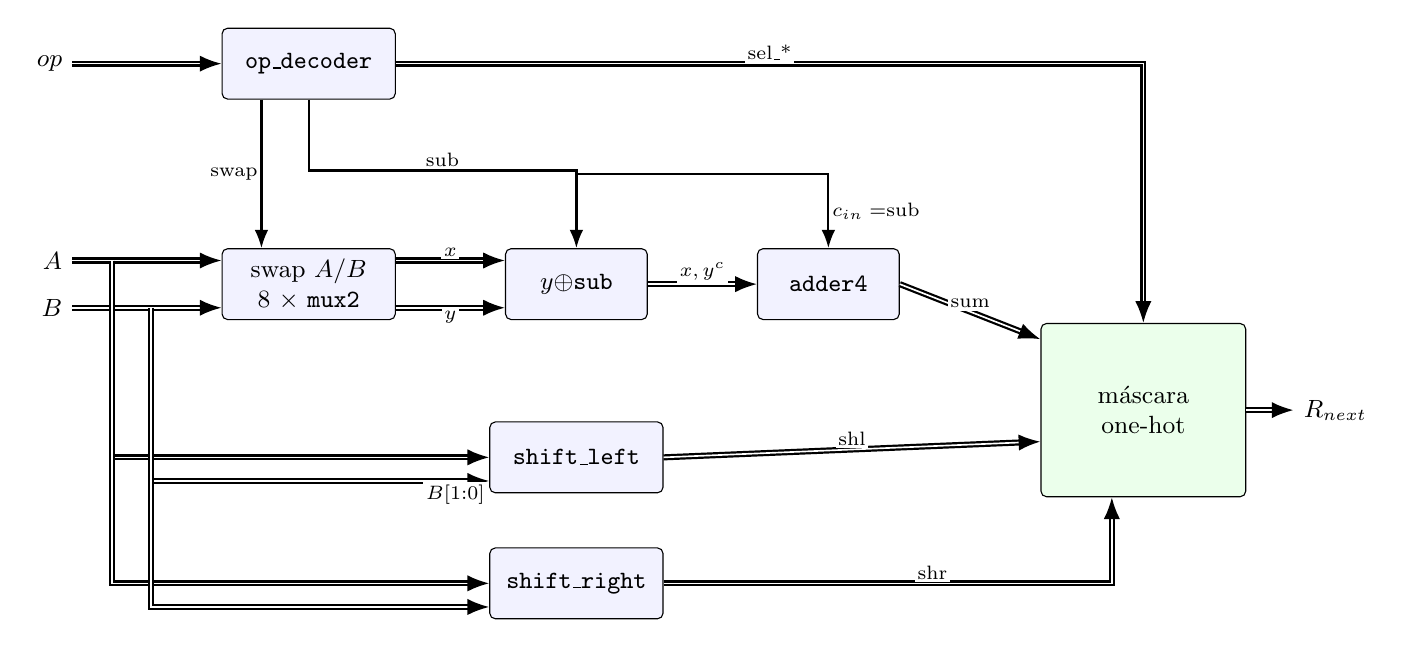
\begin{tikzpicture}[font=\small,
  blk/.style={draw,rounded corners=2pt,minimum height=9mm,align=center,fill=blue!5},
  ar/.style={-Latex,thick}, bus/.style={-Latex,thick,double}, lbl/.style={font=\scriptsize,fill=white,inner sep=1pt}]
\node[blk,minimum width=22mm] (dec) at (0,2.8) {\sig{op\_decoder}};
\node[blk,minimum width=22mm] (swap) at (0,0) {swap $A/B$\\8 $\times$ \sig{mux2}};
\node[blk,minimum width=18mm] (xr) at (3.4,0) {$y\oplus$\sig{sub}};
\node[blk,minimum width=18mm] (add) at (6.6,0) {\sig{adder4}};
\node[blk,minimum width=22mm] (shl) at (3.4,-2.2) {\sig{shift\_left}};
\node[blk,minimum width=22mm] (shr) at (3.4,-3.8) {\sig{shift\_right}};
\node[blk,minimum width=26mm,minimum height=22mm,fill=green!8] (mx) at (10.6,-1.6) {máscara\\one-hot};
\draw[bus] (-3,2.8) node[left]{$op$} -- (dec.west);
\draw[bus] (-3,0.3) node[left]{$A$} -- ($(swap.west)+(0,0.3)$);
\draw[bus] (-3,-0.3) node[left]{$B$} -- ($(swap.west)+(0,-0.3)$);
\draw[bus] ($(swap.east)+(0,0.3)$) -- node[lbl,above]{$x$} ($(xr.west)+(0,0.3)$);
\draw[bus] ($(swap.east)+(0,-0.3)$) -- node[lbl,below]{$y$} ($(xr.west)+(0,-0.3)$);
\draw[bus] (xr.east) -- node[lbl,above]{$x,y^c$} (add.west);
\draw[bus] (add.east) -- node[lbl,above]{sum} ($(mx.west)+(0,0.9)$);
\draw[bus] (-2.5,0.3) |- (shl.west);
\draw[bus] (-2.5,0.3) |- (shr.west);
\draw[bus] (-2.0,-0.3) |- ($(shl.west)+(0,-0.3)$) node[lbl,pos=0.95,below]{$B[1{:}0]$};
\draw[bus] (-2.0,-0.3) |- ($(shr.west)+(0,-0.3)$);
\draw[bus] (shl.east) -- node[lbl,above]{shl} ($(mx.west)+(0,-0.4)$);
\draw[bus] (shr.east) -| node[lbl,pos=0.3,above]{shr} ($(mx.south)+(-4mm,0)$);
\draw[bus] (dec.east) -- node[lbl,above]{sel\_*} (10.6,2.8) -- (mx.north);
\draw[ar] (dec.south) -- ++(0,-0.9) -| node[lbl,pos=0.25,above]{sub} (xr.north);
\draw[ar] (3.4,1.4) -| node[lbl,pos=0.75,right]{$c_{in}=$sub} (add.north);
\draw[ar] ($(dec.south)+(-0.6,0)$) -- node[lbl,left]{swap} ($(swap.north)+(-0.6,0)$);
\draw[bus] (mx.east) -- ++(0.6,0) node[right]{$R_{next}$};
\end{tikzpicture}}
\caption{Estructura de la ALU (\sig{alu.v}).}
\label{fig:alu}
\end{figure}

\begin{lstlisting}[language=Verilog]
// alu.v (extracto)
or  c0 (sub,  sel_sub, sel_rsub);
buf c1 (swap, sel_rsub);
mux2 sx0 (a[0], b[0], swap, x[0]);   // ... bits 1..3
mux2 sy0 (b[0], a[0], swap, y[0]);   // ... bits 1..3
xor k0 (yc[0], y[0], sub);           // ... bits 1..3
adder4 add (x, yc, sub, sum, cout);  // cout descartado -> modulo 16
shift_left  sl (a, b[1:0], shl);
shift_right sr (a, b[1:0], shr);
and ga0 (m_add[0], sum[0], sel_add);  and gs0 (m_sub[0], sum[0], sel_sub);
and gr0 (m_rsub[0], sum[0], sel_rsub); and gl0 (m_shl[0], shl[0], sel_shl);
and gh0 (m_shr[0], shr[0], sel_shr);   // ... bits 1..3
or  f0 (r[0], m_add[0], m_sub[0], m_rsub[0], m_shl[0], m_shr[0]);
\end{lstlisting}

\subsection{Barrel shifter}

\begin{lstlisting}[language=Verilog]
// shift_left.v
mux2 p3 (a[3], a[2], sh[0], t[3]);   mux2 q3 (t[3], t[1], sh[1], y[3]);
mux2 p2 (a[2], a[1], sh[0], t[2]);   mux2 q2 (t[2], t[0], sh[1], y[2]);
mux2 p1 (a[1], a[0], sh[0], t[1]);   mux2 q1 (t[1], 1'b0, sh[1], y[1]);
mux2 p0 (a[0], 1'b0, sh[0], t[0]);   mux2 q0 (t[0], 1'b0, sh[1], y[0]);
\end{lstlisting}

\subsection{Contador y máquina de estados}

\begin{lstlisting}[language=Verilog]
// counter4.v (cadena de subida, bit 1 como ejemplo)
xor ib (n_inc[1], q[1], q[0]);   and ic (c2, q[0], q[1]);   // c[1] = q[0]
and s0 (inc_ok, en, inc);  not s1 (ninc, inc);  and s2 (dec_raw, dec, ninc);
and s3 (dec_ok, en, dec_raw);                    nor s4 (hold, inc_ok, dec_ok);
and g10 (m_inc[1], n_inc[1], inc_ok);  and g11 (m_dec[1], n_dec[1], dec_ok);
and g12 (m_hold[1], q[1], hold);       or  g13 (m_or[1], m_inc[1], m_dec[1], m_hold[1]);
and r2  (d[1], m_or[1], nrst);
always @(posedge clk) q <= d;   // unico bloque secuencial
\end{lstlisting}

\begin{lstlisting}[language=Verilog]
// fsm_control.v
not v1 (ns1, q1);  not v0 (ns0, q0);
and e0 (en_op, ns1, ns0);  and e1 (en_A, ns1, q0);  and e2 (en_B, q1, ns0);  and e3 (en_R, q1, q0);
and c0 (sel_op2, usar_anterior, en_B);   or  c1 (any_conf, confirmar, usar_anterior);
and c2 (load_R,  en_B, any_conf);        or  c3 (avanzar,  confirmar, sel_op2);
xor p1 (n1, q1, q0);  buf p0 (n0, ns0);
mux2 h1 (q1, n1, avanzar, m1);  mux2 h0 (q0, n0, avanzar, m0);
and r1 (d1, m1, nrst);  and r2 (d0, m0, nrst);
\end{lstlisting}

\subsection{Valor absoluto y 7 segmentos}

\begin{lstlisting}[language=Verilog]
// abs4.v
xor x0 (x[0], v[0], v[3]);
xor x1 (x[1], v[1], v[3]);
xor x2 (x[2], v[2], v[3]);
adder4 inc ({1'b0, x[2:0]}, 4'b0000, v[3], d, cout);
\end{lstlisting}

\begin{lstlisting}[language=Verilog]
// seg7_decoder.v (productos compartidos y dos salidas de ejemplo)
and q0 (p_n2n0, n2, n0);   and q3 (p_d2n1, D2, n1);   and q4 (p_d2n0, D2, n0);
or  sa (seg[6], p_n2n0, D1, p_d2d0);              // a
or  q9 (e_or, n2, D1);   and se (seg[2], n0, e_or); // e
or  sg (seg[0], p_n2d1, p_d2n1, p_d2n0, D3);       // g
\end{lstlisting}

\subsection{Conteo de compuertas por módulo}

Cada módulo documenta su propio conteo en el encabezado del archivo:

\begin{table}[H]
\centering\small
\begin{tabular}{@{}llll@{}}
\toprule
\textbf{Módulo} & \textbf{Compuertas} & \textbf{FF} & \textbf{Detalle} \\
\midrule
\sig{mux2}         & 4  & -- & 1 NOT + 2 AND + 1 OR \\
\sig{full\_adder}  & 5  & -- & 2 XOR + 2 AND + 1 OR \\
\sig{adder4}       & 20 & -- & 4 $\times$ \sig{full\_adder} \\
\sig{shift\_left}/\sig{shift\_right} & 32 c/u & -- & 8 $\times$ \sig{mux2} \\
\sig{op\_decoder}  & 9  & -- & 3 NOT + 6 AND$_3$ \\
\sig{abs4}         & --  & -- & 3 XOR + \sig{adder4} (20) \\
\sig{seg7\_decoder}& 20 & -- & 3 NOT + 10 AND + 7 OR \\
\sig{reg4}         & 21 & 4  & 4 $\times$ \sig{mux2} + 4 AND reset + 1 NOT \\
\sig{reg4\_ini}    & 16 & 4  & 4 $\times$ \sig{mux2}, sin reset \\
\sig{dash\_s0}     & 9  & -- & 6 AND + 2 OR + 1 NOT \\
\sig{por}          & --  & 4  & 4 buf + 1 NOT \\
\sig{fsm\_control} & 24 & 2  & 2 NOT + 2 \sig{mux2} + $\sim$10 compuertas de control \\
\sig{debounce}     & 17 & 4  & 3 \sig{mux2} + AND$_3$ + OR$_3$ + AND + OR + NOT \\
\sig{edge\_detect} & --  & 1  & NOT + AND \\
\sig{boton}        & 20 & 5  & \sig{debounce} + \sig{edge\_detect} \\
\sig{prescaler}    & 44 & 15 & 1 NOT + 14 XOR + 14 AND + 15 AND reset \\
\bottomrule
\end{tabular}
\caption{Conteo de compuertas primitivas propias de cada módulo (según su propio encabezado en el código); no incluye los submódulos que instancia. \sig{alu}, \sig{counter4} y \sig{op\_selector} se describen por estructura en las secciones anteriores en vez de un total único.}
\end{table}

El resultado de síntesis real (174 celdas lógicas del iCE40 HX1K, sección 1.7) es la cifra que importa para la FPGA: la diferencia con la suma de compuertas primitivas se debe a que cada \sig{SB\_LUT4} del dispositivo absorbe varias compuertas al mapear la netlist.

\end{document}
